\documentclass[11pt,reqno]{amsart}

\usepackage[T1]{fontenc}
\usepackage[utf8]{inputenc}
\usepackage{amsmath,amssymb,amsthm,mathtools}
\usepackage{graphicx}
\usepackage{booktabs}
\usepackage[margin=1in]{geometry}
\emergencystretch=3em
\usepackage[protrusion=true,expansion=false]{microtype}
\usepackage{xcolor}
\usepackage[colorlinks=true,linkcolor=blue!55!black,citecolor=green!45!black,urlcolor=blue!55!black]{hyperref}

\theoremstyle{plain}
\newtheorem{theorem}{Theorem}[section]
\newtheorem{lemma}[theorem]{Lemma}
\newtheorem{proposition}[theorem]{Proposition}
\newtheorem{corollary}[theorem]{Corollary}
\theoremstyle{definition}
\newtheorem{definition}[theorem]{Definition}
\newtheorem{remark}[theorem]{Remark}
\newtheorem{observation}[theorem]{Observation}

\DeclareMathOperator{\tr}{tr}
\DeclareMathOperator{\adj}{adj}
\DeclareMathOperator{\Hess}{Hess}
\newcommand{\R}{\mathbb{R}}
\newcommand{\C}{\mathbb{C}}
\newcommand{\Sph}{\mathbb{S}}
\newcommand{\calT}{\mathcal{T}}
\newcommand{\calD}{\mathcal{D}}
\newcommand{\Fz}{F_{z}}
\newcommand{\eps}{\varepsilon}
\newcommand{\ie}{i.e.\ }
\newcommand{\eg}{e.g.\ }

\begin{document}

\title[Exact fiber elimination for the PCR3BP convexity gates]{Exact fiber elimination for the Levi--Civita convexity gates of the planar restricted three-body problem, with a global convexity reconnaissance}

\author{C\'esar Augusto Grisa}
\address{Instituto de Computa\c{c}\~ao, Universidade Federal Fluminense, Niter\'oi, RJ, Brazil}
\email{cagrisa@id.uff.br}

\date{\today}

\subjclass[2020]{Primary 70F07; Secondary 37J06, 53A07, 68W30}
\keywords{Restricted three-body problem, Levi--Civita regularization, strict convexity, global surface of section, Birkhoff conjecture, computer-assisted proof}

\begin{abstract}
Computer-assisted strict-convexity certification of the regularized energy surfaces of the planar circular restricted three-body problem (PCR3BP) reduces to the simultaneous positivity of two scalar \emph{gates}, $T$ and $D$, over a three-dimensional domain: a two-dimensional Levi--Civita base together with a fiber angle $\phi\in\Sph^1$. We prove four exact algebraic identities giving an exact tangential fiber minimum and a rigorous determinant lower bound without a fiber sweep. The tangential gate satisfies $\min_\phi T = \calT$ with $\calT$ an explicit function of the base alone, attained at a computable angle; the curvature-determinant gate admits an exact five-term harmonic decomposition whose second-harmonic amplitude is $128F^2 s$ for the structure matrices at hand, yielding the rigorous lower bound $D\ge \calD := A_0-\sqrt{A_1^2+B_1^2}-128F^2 s$, which is sharp on the collar. Thus the tangential condition is reduced exactly from three variables to two, while the determinant condition is replaced by a sufficient two-variable condition. All identities are confirmed by an exact symbolic audit whose residuals vanish identically. As a numerical spot check, pointwise evaluations of the reduced gates are reported near the Earth--Moon mass ratio (the regularized component being the Moon's); this is not an interval certificate. Using the reduced gates we compute a global reconnaissance of Levi--Civita convexity across the mass--energy plane, parametrized by the mass fraction $m_r$ of the regularized primary. In the numerical scans near the critical energy, the apparent non-convex window is large and asymmetric: at $\Delta c=10^{-4}$ the apparent window begins near $m_r\approx 0.045$ and includes the largest sampled fraction $m_r=0.999$, so the scans suggest LC-convexity there only for components regularized at a sufficiently light primary. The computed heavy-side non-convexity persists at the sampled masses approaching the rotating-Kepler limit; it does not extend an Euler-model theorem. We record a numerical observation that the non-convexity region avoids the coordinate axes in the sampled comparable-mass cases and forms lateral lobes on which the failure is a single simple fold---one negative principal curvature, the tangential gate staying positive---while the base remains radially star-shaped; and we discuss the limits of inferring dynamics from embedding convexity. A refinement of the reconnaissance down to energy offsets of $10^{-7}$ suggests that even the Moon component of the Earth--Moon system ($m_r\approx 0.0122$) loses LC-convexity on an ultrathin shell of width $\approx 9.5\times 10^{-6}$ above the critical energy, where the Lagrange point enters the surface; for the Earth component ($m_r\approx 0.9878$), the scans suggest a macroscopic near-critical non-convexity window and positive sampled gates at offsets $\Delta c\gtrsim 1.2\times 10^{-2}$. This numerically locates a possible limitation of the LC route near the critical limit. (This is version~2 of the paper: it corrects a mass-convention mislabeling and a scanning-heuristic flaw of version~1; see the erratum note in Section~\ref{sec:map}.)
\end{abstract}

\maketitle

\section{Introduction}\label{sec:intro}

\subsection{Background}
Let $\mu\in(0,1)$ be the mass ratio of the two primaries of the planar circular restricted three-body problem (PCR3BP). Below the first critical energy, the regularized bounded components are contact manifolds diffeomorphic to $\mathbb{R}P^3$, with Levi--Civita double covers diffeomorphic to $\Sph^3$~\cite{AFKP}. A central structural question, going back to Birkhoff~\cite{Birkhoff}, is whether the retrograde periodic orbit bounds a disk-like global surface of section, interpreted rationally on the quotient. Hofer, Wysocki and Zehnder~\cite{HWZ} establish the existence of a disk-like global section for a closed strictly convex hypersurface in $\R^4$. On a lens space, Hryniewicz and Salom\~ao~\cite{HS} obtain rational open books from dynamical convexity when the proposed binding is a $p$-unknot with rational self-linking number $-1/p$. Identifying a prescribed orbit as the binding requires these additional topological conditions; it does not follow from a local convexity test alone.

The standard double cover is the Levi--Civita (LC) regularization~\cite{LeviCivita}, which represents the bounded component by a compact hypersurface $\Sigma_{\mu,c}=\{K_c=0\}\subset\R^4\cong\C^2$. Convexity depends on the chosen embedding. Kim~\cite{Kim} studies the mechanical Euler problem of two fixed centers: his Theorem~1.1 concerns an elliptic-coordinate embedding, whereas Theorem~1.3 concerns non-convexity of its standard LC image. Remark~1.2 discusses small rotation perturbations. These statements are not a mass threshold for the full rotating PCR3BP; the proposed comparison is qualified in Section~\ref{sec:map}.

Convexity tests for Hamiltonian energy levels were developed earlier by Salom\~ao~\cite{Salomao2004}, for mechanical systems including non-regular levels. In celestial mechanics, global sections in suitable lunar parameter ranges were constructed by Albers, Fish, Frauenfelder, Hofer and van Koert~\cite{AFFHvK}; dynamical convexity and convex embeddings of the rotating Kepler problem were studied in~\cite{AFFvK,FKZ}. Rational global sections with prescribed bindings also arise in~\cite{HLS,HS}. More recently, Liu and Salom\~ao~\cite{LSPCR} construct finite energy foliations near the first critical level and prove Birkhoff's retrograde-orbit conclusion for mass ratios sufficiently close to $1/2$ at all subcritical energies; their Hill-problem work~\cite{LSHill} establishes the corresponding subcritical conclusion and near-critical foliations in that model. These results motivate approaches beyond convexity of one fixed LC embedding. The present contribution remains the algebraic elimination of the fiber variable and a separately identified numerical reconnaissance.

\subsection{The computational bottleneck}
A computer-assisted convexity check on a fixed parameter box can proceed by verifying, with interval arithmetic, that a pair of scalar \emph{gates} $T$ and $D$ are strictly positive at every point of the regularized surface. After the LC reduction the surface fibers over a compact two-dimensional base $z=(z_1,z_2)$ by an angle $\phi\in\Sph^1$, so each gate is a function of the three real variables $(z_1,z_2,\phi)$ (with the parameters $\mu,c$ fixed). The angular variable multiplies the cost of certification: every base cell must be checked against the whole circle of fiber directions, and the interval enclosures of trigonometric expressions inflate the bounds. Eliminating $\phi$ analytically gives an exact two-variable minimum for $T$ and a sufficient two-variable lower bound for $D$, removing the fiber sweep when these reduced positivity conditions hold.

\subsection{Contributions}
This paper makes the following contributions.
\begin{enumerate}
\item[(i)] \textbf{Exact fiber elimination.} We prove four algebraic identities (Lemmas~\ref{lem:T}--\ref{lem:amp}) that remove the fiber variable from the tangential test and yield a sufficient determinant test on the two base variables $z$. For the tangential gate the reduction is an exact minimum, $\min_\phi T=\calT(z)$, attained at an explicit angle. For the curvature-determinant gate we obtain an exact harmonic decomposition and a rigorous, collar-sharp lower bound $D\ge\calD(z)$. Section~\ref{sec:elimination}.
\item[(ii)] \textbf{Symbolic certification.} Every identity is confirmed by an exact computer-algebra audit whose eight residuals vanish identically; the audit is short, deterministic, and included in the reproducibility package (Appendix~\ref{app:audit}).
\item[(iii)] \textbf{Application.} Pointwise evaluations of the reduced gates are reported near the Earth--Moon mass ratio as a reproducible numerical spot check (Section~\ref{sec:earthmoon}).
\item[(iv)] \textbf{Global reconnaissance.} Using the reduced gates we compute a floating-point map of LC-convexity across the mass--energy plane, in the mass fraction $m_r$ of the regularized primary. At the sampled near-critical offsets, the apparent non-convex window begins near $m_r\approx 0.045$ and includes $m_r=0.999$, the largest sampled fraction; no negative determinant value is found for $\Delta c\gtrsim 0.03$ at the mass ratios scanned (Section~\ref{sec:map}).
\item[(v)] \textbf{A dynamical-relevance observation.} We record numerical evidence that the non-convexity region avoids the coordinate axes in the sampled comparable-mass cases and that, on the lateral lobes where it lives, the failure is a single simple fold on a base that stays radially star-shaped; and we discuss the remaining limitations of this embedding-based test (Sections~\ref{sec:relevance}--\ref{sec:outlook}).
\end{enumerate}
Contributions (i)--(ii) are rigorous; (iii) is a finite numerical spot check, not an interval certification; (iv)--(v) are floating-point reconnaissance and are labeled as such throughout.

\section{The regularized surface and the convexity gates}\label{sec:setup}

\subsection{Levi--Civita coordinates}
In rotating coordinates centered at the primary being regularized, with the other primary at $(1,0)$, pass to Levi--Civita coordinates $z=(z_1,z_2)\in\R^2$ via $q=2\bar z^2$. Writing $s=|z|^2=z_1^2+z_2^2$ and $a=z_1^2-z_2^2$, the regularized defining function for the bounded component takes the form
\begin{equation}\label{eq:F}
F(z)=1-\mu+\frac{2\mu s}{\sqrt{1-4a+4s^2}}-2cs+\mu^2 s+4s^3-4\mu s a,
\end{equation}
where $c$ is one half of the Jacobi constant. Let $B_{\mu,c}\subset\R^2$ denote the relevant closed bounded base component on which $F\ge0$. Its boundary $\partial B_{\mu,c}$, given by $F=0$, is the locus called the \emph{collar} in this paper. This one-dimensional boundary must not be confused with the three-dimensional regularized hypersurface $\Sigma_{\mu,c}=\{K_c=0\}\subset\R^4$ introduced in Section~\ref{sec:intro}. The hypersurface projects onto $B_{\mu,c}$; the fiber is a circle parametrized by $\phi$ when $F>0$ and collapses at the collar. Note that $F$ depends on $z$ only through the pair $(s,a)$; this is used repeatedly below.

\begin{remark}[Mass convention]\label{rem:mass}
In~\eqref{eq:F} the parameter $\mu$ is the mass fraction of the \emph{distant} primary, located at $q=(1,0)$; the \emph{regularized} primary, at the origin, has mass fraction $m_r=1-\mu$. Indeed, writing $\Omega(q)=\tfrac12|q-b|^2+(1-\mu)/|q|+\mu/|q-e|$ for the effective potential of the pair with mass $1-\mu$ at the origin, mass $\mu$ at $e=(1,0)$ and barycentre $b=(\mu,0)$, the substitution $q=2\bar z^2$ gives the exact identity $F=|q|\,(\Omega(q)-c)$, reproducing~\eqref{eq:F} term by term ($\sqrt{1-4a+4s^2}=|q-e|$, $\mu^2 s=\tfrac12\mu^2|q|$ from the barycentric offset, $-4\mu sa=-\mu q_1|q|$); the identity is verified symbolically in the reproducibility package. Version~1 of this paper mislabeled $m_r$ as $\mu$ itself in the reconnaissance sections; all component attributions below use the corrected convention.
\end{remark}

\subsection{The two gates}\label{sec:gates}
We use the following scalar-gate formulation of the LC convexity check. Its data are encoded by the symmetric $2\times2$ matrix pencil
\begin{equation}\label{eq:L}
L(z,\phi)=-\tfrac12\Hess F(z)+\sqrt{F}\,\bigl(\cos\phi\,M_1(z)+\sin\phi\,M_2(z)\bigr),
\end{equation}
where $\phi\in\Sph^1$ is the fiber angle and $M_1,M_2$ are the fixed structure matrices arising from the second-order data of the LC map,
\begin{equation}\label{eq:M}
M_1=\begin{pmatrix}-4z_2&-4z_1\\-4z_1&-12z_2\end{pmatrix},
\qquad
M_2=\begin{pmatrix}12z_1&4z_2\\4z_2&4z_1\end{pmatrix}.
\end{equation}
The two scalar \emph{gates} include both the gradient and the matrix data:
\begin{align}
T(z,\phi)&:=|\Fz|^2+4F\,\tr L(z,\phi),\label{eq:T}\\
D(z,\phi)&:=\Fz^{\!\top}\adj\!\bigl(L(z,\phi)\bigr)\Fz+4F\,\det L(z,\phi),\label{eq:D}
\end{align}
where $\Fz=(\partial_{z_1}F,\partial_{z_2}F)^\top$ is the base gradient and $\adj$ denotes the adjugate. For $F>0$, define
\[
C(z,\phi):=L(z,\phi)+\frac{\Fz\Fz^{\!\top}}{4F}.
\]
The rank-one determinant identity gives $T=4F\tr C$ and $D=4F\det C$. Thus $T,D>0$ is equivalent to positive-definiteness of $C$, not necessarily of $L$. At $F=0$ we use the original, nonsingular gate formulas~\eqref{eq:T}--\eqref{eq:D}. The certificate criterion is that
\[
T(z,\phi)>0\quad\text{and}\quad D(z,\phi)>0\qquad\text{for all }z\text{ in the base and all }\phi\in\Sph^1
\]
are the scalar-gate positivity conditions used for strict-convexity certification of $\Sigma_{\mu,c}$. The derivation from the second fundamental form is not the contribution of this paper; here we take~\eqref{eq:T}--\eqref{eq:D} as the starting point and prove the exact minimum over $\phi$ for $T$, together with an exact harmonic decomposition and a rigorous, fiber-independent lower bound for $D$.

\section{Exact fiber elimination}\label{sec:elimination}

Throughout this section $\mu,c$ are fixed and $z$ ranges over $B_{\mu,c}$, where $F\ge 0$ (the closed component bounded by the collar), so that $\sqrt{F}$ is real.

\subsection{The tangential gate}

\begin{lemma}[Closed form for the tangential gate]\label{lem:T}
With $T$ as in~\eqref{eq:T} and $L$ as in~\eqref{eq:L},
\begin{equation}\label{eq:Tgap}
T(z,\phi)=\calT(z)+64\,F^{3/2}\bigl(\sqrt{s}-z_2\cos\phi+z_1\sin\phi\bigr),
\qquad
\calT(z):=|\Fz|^2-2F\,\Delta F-64\,F^{3/2}\sqrt{s},
\end{equation}
where $\Delta F=\tr\Hess F$. The bracket in~\eqref{eq:Tgap} is nonnegative, and
\begin{equation}\label{eq:Tmin}
\min_{\phi\in\Sph^1} T(z,\phi)=\calT(z),
\end{equation}
attained, for $s>0$, at $(\cos\phi^\ast,\sin\phi^\ast)=(z_2,-z_1)/\sqrt{s}$. If $s=0$, then $z=0$ and the angular term has zero amplitude, so every angle is minimizing. Every angle is also minimizing on the collar $F=0$. Consequently the tangential gate holds on the whole fiber, $T(z,\phi)>0$ for all $\phi$, if and only if $\calT(z)>0$.
\end{lemma}

\begin{proof}
From~\eqref{eq:M}, $\tr M_1=-4z_2-12z_2=-16z_2$ and $\tr M_2=12z_1+4z_1=16z_1$. Hence, by~\eqref{eq:L},
\[
\tr L=-\tfrac12\Delta F+\sqrt{F}\,(-16z_2\cos\phi+16z_1\sin\phi),
\]
and substituting into~\eqref{eq:T},
\[
T=|\Fz|^2-2F\,\Delta F+64\,F^{3/2}(-z_2\cos\phi+z_1\sin\phi).
\]
Adding and subtracting $64F^{3/2}\sqrt{s}$ gives~\eqref{eq:Tgap}. The map $\phi\mapsto -z_2\cos\phi+z_1\sin\phi$ is a sinusoid of amplitude $\sqrt{z_1^2+z_2^2}=\sqrt{s}$, so its minimum over $\Sph^1$ is $-\sqrt{s}$, whence the bracket $\sqrt{s}-z_2\cos\phi+z_1\sin\phi$ ranges over $[0,2\sqrt{s}]$ and is nonnegative; its minimum $0$ is attained when $-z_2\cos\phi+z_1\sin\phi=-\sqrt{s}$; for $s>0$, this is attained at $(\cos\phi^\ast,\sin\phi^\ast)=(z_2,-z_1)/\sqrt{s}$. Since $F\ge0$, the term $64F^{3/2}(\cdot)$ is nonnegative and vanishes at this angle. If $s=0$ or $F=0$, the angular contribution is identically zero. This proves~\eqref{eq:Tmin} in all cases. The amplitude claim is the exact identity
\begin{equation}\label{eq:sq}
s-(-z_2\cos\phi+z_1\sin\phi)^2=(z_1\cos\phi+z_2\sin\phi)^2,
\end{equation}
a perfect square, which shows $(-z_2\cos\phi+z_1\sin\phi)^2\le s$ for every $\phi$.
\end{proof}

The point of Lemma~\ref{lem:T} is that~\eqref{eq:Tmin} is an \emph{exact minimum}, not a bound: the tangential gate is certified over the whole fiber precisely when the two-variable surrogate $\calT$ is positive. No fiber sweep is required.

\begin{lemma}[Base-invariant reduction]\label{lem:sa}
The quantities $|\Fz|^2$ and $\Delta F$ are functions of $(s,a)$ alone; explicitly,
\begin{align}
|\Fz|^2&=4s\,F_s^2+8a\,F_sF_a+4s\,F_a^2,\label{eq:grad}\\
\Delta F&=4s\,F_{ss}+8a\,F_{sa}+4s\,F_{aa}+4F_s,\label{eq:lap}
\end{align}
where subscripts denote partial derivatives of $F$ regarded as a function of $(s,a)$. In particular $\calT=\calT(s,a;c)$.
\end{lemma}

\begin{proof}
Since $F$ depends on $z$ through $s=z_1^2+z_2^2$ and $a=z_1^2-z_2^2$, the chain rule gives $\partial_{z_1}F=2z_1(F_s+F_a)$ and $\partial_{z_2}F=2z_2(F_s-F_a)$. Therefore
\[
|\Fz|^2=4z_1^2(F_s+F_a)^2+4z_2^2(F_s-F_a)^2
=4(z_1^2+z_2^2)(F_s^2+F_a^2)+8(z_1^2-z_2^2)F_sF_a,
\]
which is~\eqref{eq:grad}. A second application of the chain rule yields $\partial_{z_1}^2F+\partial_{z_2}^2F=4sF_{ss}+8aF_{sa}+4sF_{aa}+4F_s$, which is~\eqref{eq:lap}. Both are functions of $(s,a)$, and by Lemma~\ref{lem:T} so is $\calT$.
\end{proof}

\begin{corollary}[Quadrant reduction]\label{cor:quad}
The reduced tangential gate $\calT$ is invariant under the reflections $(z_1,z_2)\mapsto(\pm z_1,\pm z_2)$. Hence the tangential gate need only be certified on a single closed quadrant of the base.
\end{corollary}

\begin{proof}
Both $s=z_1^2+z_2^2$ and $a=z_1^2-z_2^2$ are invariant under each sign change of $z_1$ or $z_2$, and $\calT$ depends on $z$ only through $(s,a)$ by Lemma~\ref{lem:sa}.
\end{proof}

Corollary~\ref{cor:quad} supplies a rigorous justification for the quadrant symmetry reduction used in practice: it is not an assumption but a consequence of the functional form of $F$.

\subsection{The curvature-determinant gate}

The elimination of $\phi$ from $D$ rests on a purely multilinear identity, valid for arbitrary symmetric $2\times2$ data, which we state and prove in that generality before specializing.

For symmetric $2\times2$ matrices $X,Y$ write $\sigma(X,Y):=\tr X\,\tr Y-\tr(XY)$ for the polarization of the determinant, so that $\det(X+Y)=\det X+\det Y+\sigma(X,Y)$; recall that for $2\times2$ matrices $\adj$ is linear.

\begin{lemma}[Harmonic decomposition of the determinant gate]\label{lem:harm}
Let $L_0,M_1,M_2$ be symmetric $2\times 2$ matrices, $g\in\R^2$, $\rho\ge0$, and $F\in\R$. Put $v=(\rho\cos\phi,\rho\sin\phi)$ and $L=L_0+v_1M_1+v_2M_2$. Then
\begin{equation}\label{eq:harm}
g^\top\adj(L)\,g+4F\det L=A_0+A_1\cos\phi+B_1\sin\phi+A_2\cos2\phi+B_2\sin2\phi,
\end{equation}
with
\begin{align*}
A_0&=g^\top\adj(L_0)g+4F\det L_0+2F\rho^2\bigl(\det M_1+\det M_2\bigr),\\
A_1&=\rho\bigl(g^\top\adj(M_1)g+4F\,\sigma(L_0,M_1)\bigr),
&
B_1&=\rho\bigl(g^\top\adj(M_2)g+4F\,\sigma(L_0,M_2)\bigr),\\
A_2&=2F\rho^2\bigl(\det M_1-\det M_2\bigr),
&
B_2&=2F\rho^2\,\sigma(M_1,M_2).
\end{align*}
\end{lemma}

\begin{proof}
By linearity of the adjugate, $\adj(L)=\adj(L_0)+v_1\adj(M_1)+v_2\adj(M_2)$, so
\[
g^\top\adj(L)g=g^\top\adj(L_0)g+v_1\,g^\top\adj(M_1)g+v_2\,g^\top\adj(M_2)g.
\]
By the polarization identity for $2\times2$ determinants applied twice,
\[
\det L=\det L_0+v_1^2\det M_1+v_2^2\det M_2+v_1\sigma(L_0,M_1)+v_2\sigma(L_0,M_2)+v_1v_2\,\sigma(M_1,M_2).
\]
Substitute $v_1=\rho\cos\phi$, $v_2=\rho\sin\phi$ and use the double-angle identities
$\cos^2\phi=\tfrac12(1+\cos2\phi)$, $\sin^2\phi=\tfrac12(1-\cos2\phi)$, $\cos\phi\sin\phi=\tfrac12\sin2\phi$.
Collecting the constant, first-harmonic and second-harmonic terms gives exactly the stated coefficients.
\end{proof}

Specializing to the LC surface, take $L_0=-\tfrac12\Hess F$, $g=\Fz$, and $\rho=\sqrt{F}$ (so that $\rho^2=F$), with $M_1,M_2$ as in~\eqref{eq:M}. Then~\eqref{eq:harm} is precisely the fiber expansion of the gate $D$ in~\eqref{eq:D}. The next lemma computes the second-harmonic amplitude for these structure matrices.

\begin{lemma}[Second-harmonic amplitude]\label{lem:amp}
For $M_1,M_2$ as in~\eqref{eq:M},
\begin{equation}\label{eq:detsum}
\det M_1+\det M_2=32s,
\qquad
(\det M_1-\det M_2)^2+\sigma(M_1,M_2)^2=(64s)^2.
\end{equation}
Consequently, with $\rho^2=F$, the second-harmonic amplitude of $D$ is
\begin{equation}\label{eq:amp}
\sqrt{A_2^2+B_2^2}=2F\rho^2\sqrt{(\det M_1-\det M_2)^2+\sigma(M_1,M_2)^2}=128\,F^2 s.
\end{equation}
\end{lemma}

\begin{proof}
Direct computation from~\eqref{eq:M} gives $\det M_1=48z_2^2-16z_1^2$ and $\det M_2=48z_1^2-16z_2^2$, whence $\det M_1+\det M_2=32(z_1^2+z_2^2)=32s$ and $\det M_1-\det M_2=-64(z_1^2-z_2^2)=-64a$. A short calculation gives $\sigma(M_1,M_2)=-128\,z_1z_2$, so
\[
(\det M_1-\det M_2)^2+\sigma(M_1,M_2)^2=4096a^2+16384z_1^2z_2^2=4096(a^2+4z_1^2z_2^2)=4096\,s^2=(64s)^2,
\]
using $a^2+4z_1^2z_2^2=(z_1^2-z_2^2)^2+4z_1^2z_2^2=(z_1^2+z_2^2)^2=s^2$. Substituting into $\sqrt{A_2^2+B_2^2}=2F\rho^2\sqrt{(\det M_1-\det M_2)^2+\sigma(M_1,M_2)^2}$ with $\rho^2=F$ gives~\eqref{eq:amp}.
\end{proof}

\begin{corollary}[Rigorous lower bound for the determinant gate]\label{cor:Dbound}
For every $\phi\in\Sph^1$,
\begin{equation}\label{eq:Dbound}
D(z,\phi)\ge \calD(z):=A_0(z)-\sqrt{A_1(z)^2+B_1(z)^2}-128\,F(z)^2 s,
\end{equation}
where $A_0,A_1,B_1$ are as in Lemma~\ref{lem:harm} with the specialization above. The bound is sharp on the collar: at $\{F=0\}$ one has $A_1=B_1=A_2=B_2=0$ and $D=\calD=\Fz^{\!\top}\adj(-\tfrac12\Hess F)\Fz$.
\end{corollary}

\begin{proof}
By Lemma~\ref{lem:harm} and the elementary bounds $\lvert A_1\cos\phi+B_1\sin\phi\rvert\le\sqrt{A_1^2+B_1^2}$ and $\lvert A_2\cos2\phi+B_2\sin2\phi\rvert\le\sqrt{A_2^2+B_2^2}=128F^2s$ (the last equality by Lemma~\ref{lem:amp}), we get $D\ge A_0-\sqrt{A_1^2+B_1^2}-128F^2s$. On the collar $F=0$: the coefficients $A_1,B_1$ carry a factor $\rho=\sqrt{F}$ and $A_2,B_2$ a factor $\rho^2=F$, so all four vanish, leaving $D=A_0=\Fz^{\!\top}\adj(-\tfrac12\Hess F)\Fz=\calD$.
\end{proof}

\subsection{The reduction theorem}

For clarity, write
\[
D_{\min}(z):=\min_{\phi\in\Sph^1}D(z,\phi).
\]
Here $D(z,\phi)$ is the determinant gate, $\calD(z)$ is its rigorous amplitude lower bound, and $D_{\min}(z)$ is its exact fiber minimum. They satisfy $\calD(z)\le D_{\min}(z)$, with equality on the collar; away from the collar equality need not hold. Combining the lemmas therefore gives an exact tangential test and a sufficient determinant test in two base variables.

\begin{theorem}[Two-dimensional sufficient criterion for the convexity gates]\label{thm:reduction}
Fix $\mu,c$ and let $z$ range over $B_{\mu,c}$. Then:
\begin{enumerate}
\item[(a)] The tangential gate holds on every fiber, $T(z,\phi)>0$ for all $\phi\in\Sph^1$, if and only if $\calT(z)>0$, where $\calT=|\Fz|^2-2F\Delta F-64F^{3/2}\sqrt s$ is a function of $(s,a)$ alone.
\item[(b)] The determinant gate holds on every fiber whenever $\calD(z)>0$, where $\calD=A_0-\sqrt{A_1^2+B_1^2}-128F^2s$; the sufficient condition $\calD>0$ is sharp on the collar, where it coincides with $D$.
\end{enumerate}
In particular, strict convexity of $\Sigma_{\mu,c}$ is certified by the two-variable conditions $\calT>0$ and $\calD>0$ over the base, with no sweep over the fiber angle.
\end{theorem}

\begin{proof}
Part (a) is Lemmas~\ref{lem:T} and~\ref{lem:sa}. Part (b) is Corollary~\ref{cor:Dbound}. The final statement combines the two, since positivity of both gates over $(z,\phi)$ certifies strict convexity by the criterion of Section~\ref{sec:setup}, and $\calT>0$ is equivalent to $\min_\phi T>0$ while $\calD>0$ implies $\min_\phi D>0$.
\end{proof}

\begin{remark}[Symbolic certification]\label{rem:audit}
Each identity above---the gap formula~\eqref{eq:Tgap}, the perfect square~\eqref{eq:sq}, the attained angle for $s>0$, the $(s,a)$ reductions~\eqref{eq:grad}--\eqref{eq:lap}, the generic harmonic decomposition~\eqref{eq:harm}, and the amplitude~\eqref{eq:detsum}---was verified by an exact computer-algebra audit. The audit forms each residual as the difference of the two sides and simplifies it to the symbol $0$; all eight residuals vanish identically. The script is deterministic, runs in seconds, and is reproduced in Appendix~\ref{app:audit}.
\end{remark}

\begin{remark}[Effect on certification cost]
The elimination removes the innermost loop of the certificate. In an interval-arithmetic setting, the fiber sweep is replaced by the evaluation of two explicit two-variable functions, and the trigonometric enclosure inflation of $\cos\phi,\sin\phi$ over $[0,2\pi)$ is eliminated in the tangential gate (where the minimum is exact) and reduced to a single amplitude bound in the determinant gate.
\end{remark}

\section{Application: an Earth--Moon numerical spot check}\label{sec:earthmoon}

As a finite numerical spot check, we evaluate the reduced gates on a small rectangle near the Earth--Moon mass ratio (by Remark~\ref{rem:mass}, with $\mu\approx0.9878$ the regularized component is the \emph{Moon's}, $m_r\approx 0.0122$),
\[
\mu\in[0.987839414390376,\;0.987859414390376],\qquad c\in[1.5995,\;1.6005].
\]
At the four parameter corners, using the sampled base grid recorded in the reproducibility checks, the minimum sampled value of $\calT$ is at least $2.29\times10^{-3}$ and the minimum sampled collar value of $\calD$ is at least $6.95\times10^{-4}$. These positive sampled values are consistent with $\calT=\min_\phi T$ and with the collar identity $\calD=D_{\min}$ at $F=0$.

This paragraph is deliberately only a numerical spot check. It does not provide an interval certificate on the full parameter rectangle, does not validate all base and fiber points, and is not used as a premise for the exact fiber-elimination identities of Section~\ref{sec:elimination}. A full certificate on a parameter rectangle would require validated evaluation of the reduced functions over a complete subdivision of that rectangle and its base domains.

\section{Global convexity reconnaissance}\label{sec:map}

We now use the reduced gates for a floating-point reconnaissance of LC-convexity across a selected mass--energy grid. This section is exploratory; its computed results are floating-point evidence and are not interval-certified. In particular, numerical values reported for $D_{\min}$ are sampled approximations to the exact minimum defined in Section~\ref{sec:elimination}, not validated enclosures.

\paragraph{Erratum note (version 2).} This section differs materially from version~1, for two compounding reasons. First, version~1 read the parameter $\mu$ of~\eqref{eq:F} as the regularized-primary mass fraction, whereas it is the distant-primary fraction (Remark~\ref{rem:mass}); all component labels are corrected here. Second, the version-1 scanner approximated $D_{\min}$ by angular sampling only at the worst base points of the amplitude bound, a heuristic that misses collar lobes when the bound is loose in the interior; this produced false ``convex'' entries at small $\mu$ (large $m_r$). The corrected scanner (worst points $\cup$ collar band) was validated against exhaustive base$\times$fiber scans at sample grid points. As a consequence, version~1's claim that the empirical boundary ``brackets Kim's $16/17$ threshold'' is withdrawn: it rested on the mislabeled variable, aided by the arithmetic coincidence $1-16/17=1/17$, and on false-convex entries. The separate model and parameter issue in the proposed comparison with Kim is addressed in Section~5.3. The corrected numerical picture is stated below; the fiber-elimination results of Sections~\ref{sec:elimination}--\ref{sec:earthmoon}, the lobe observations of Section~\ref{sec:relevance} (comparable masses, where the heuristic was reliable), and the ``convex for $\Delta c\gtrsim 0.03$'' statement are unaffected.

\subsection{Method}
For a grid of mass ratios and subcritical energies we compute the reduced tangential surrogate $\calT$ and, for the determinant gate, a sampled approximation to $D_{\min}$ by evaluating the exact degree-two trigonometric polynomial of Lemma~\ref{lem:harm} on a dense angular sample over the union of the worst base points of the amplitude bound $\calD$ \emph{and} the entire collar band (the outermost radial rows on every ray; the bound is exact at $F=0$, but may be conservative at nearby interior points). The harmonic formula is exact, but minimizing it over a finite angular sample is not exact minimization over the circle. Positive sampled values alone do not certify positivity over the full fiber or base. The collar band is essential: because $\calD$ is loose in the interior, its worst points can all be interior while the true minimum of $D$ sits on the collar; evaluating at the worst points alone (as version~1 did) produces false ``convex'' entries precisely in that situation. The first critical energy $c_{L_1}(\mu)$ is located by robust bisection between the primaries; as a sanity check the equal-mass value is recovered as $c_{L_1}=2.000000$. The grid spans sixteen mass values (including both Earth--Moon components, $\mu=0.987849\ldots$ and $\mu=0.012151\ldots$) and seven energy offsets $\Delta c=c-c_{L_1}$; the validation script \texttt{audit/v130\_validation.py} cross-checks nine selected sign conditions on a specified finite base$\times$fiber grid, without the worst-point heuristic; it does not validate every numerical value quoted in the paper.

\subsection{The non-convexity window}
The computed tangential surrogate $\calT$ is positive at the sampled points. The determinant gate, by contrast, has negative sampled values in a large, asymmetric near-critical window: writing $m_r=1-\mu$ for the regularized-primary mass fraction, at $\Delta c=10^{-4}$ the computed approximation to $D_{\min}$ is negative for every grid value $m_r\ge 0.059$ up to and including $m_r=0.999$, and positive for $m_r\le 0.03$; a dedicated high-resolution scan places the boundary at $m_r\approx 0.045$ (negative at $m_r=0.05$, $D_{\min}\approx-4\times10^{-6}$; positive at $m_r=0.04$). Thus the scans suggest near-critical LC-convexity only for components regularized at a sufficiently light primary; this is not a certified classification. The window shrinks from the light side as the energy recedes from critical and is empty for $\Delta c\gtrsim 0.03$ at every mass ratio scanned; the heavy side persists longest (at $\Delta c=10^{-2}$ only $m_r\in\{0.9,0.95,0.98\}$ remain negative on the grid). On the heavy side the lobe depth decreases toward the rotating-Kepler limit ($D_{\min}\approx-0.58$ at $m_r=0.999$, $\Delta c=10^{-4}$), but these data do not establish a limiting value as $m_r\to1$. At the sampled points the observed failure is of the determinant gate, while the tangential gate stays positive. Figure~\ref{fig:map} shows the resulting phase map.

\begin{figure}[t]
\centering
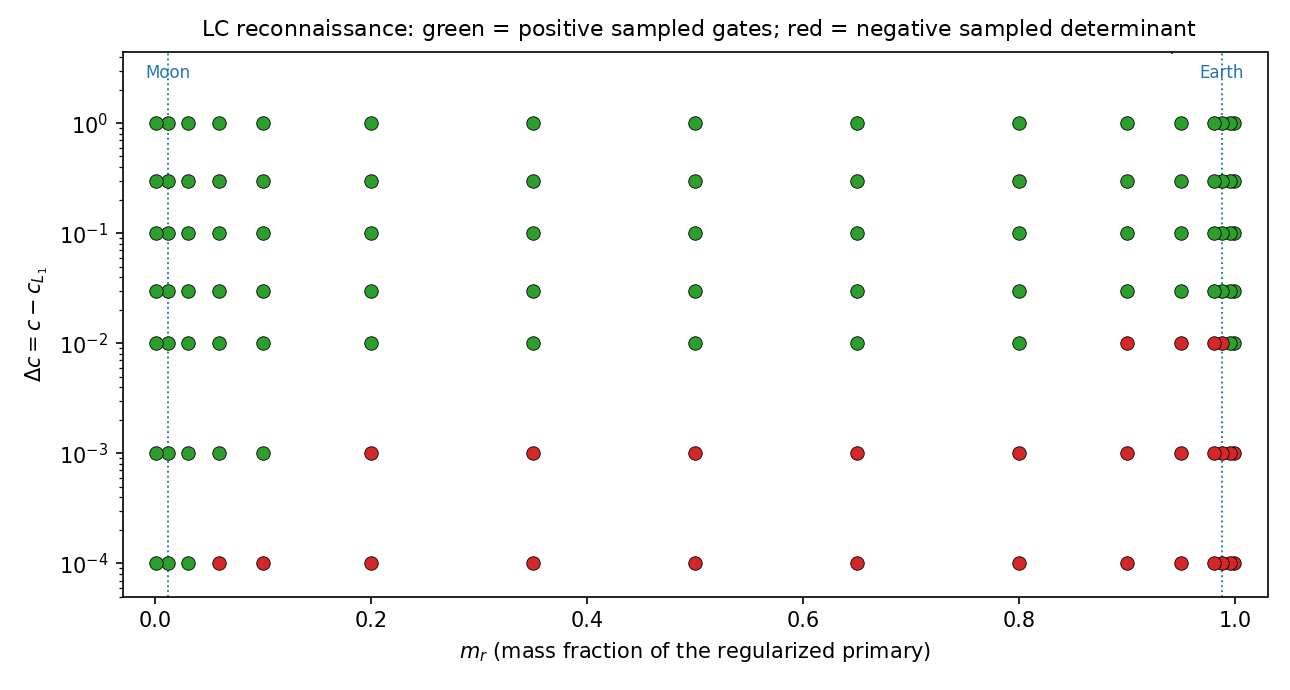
\includegraphics[width=0.86\textwidth]{figures/phase_map.png}
\caption{Floating-point reconnaissance of LC-convexity in the regularized-primary fraction $m_r$ (Remark~\ref{rem:mass}). Green markers: no negative gate value detected by the sampling procedure. Red markers: a sampled determinant value is negative. The Earth and Moon fractions are indicated. These classifications are not interval certificates. No threshold from the Euler problem is asserted for this rotating-model plot; see Section~5.3. The Moon component's smaller near-critical offsets are examined in Section~\ref{subsec:shell}.}
\label{fig:map}
\end{figure}

\subsection{Cross-check against Kim's threshold}
The proposed cross-check is not a validation for the rotating model. Kim's Theorem~1.3~\cite{Kim} concerns the Euler problem and uses the distant-primary fraction $\mu_K$: its condition $\mu_K<16/17$ corresponds to regularized-primary fraction $1-\mu_K>1/17$, not $m_r<16/17$. More importantly, that Hamiltonian lacks the PCR3BP rotation term. We therefore withdraw the earlier direct threshold comparison and remove its marker from Figure~\ref{fig:map}. The sampled boundary near $m_r\approx0.045$ and the values through $m_r=0.999$ remain numerical findings for~\eqref{eq:F}, with no theorem-based validation inferred from Kim's threshold.

\subsection{The Earth--Moon system}
The two components behave very differently. The Moon component ($m_r=0.0122$) lies below the observed light-side boundary and has positive sampled gate values at every energy offset scanned in the map ($\Delta c\ge 10^{-4}$); this is the component used in the numerical spot check of Section~\ref{sec:earthmoon}, at offsets around $\Delta c\approx 5.7\times10^{-3}$. The Earth component ($m_r=0.9878$), by contrast, sits inside the heavy-side window: its sampled determinant is negative at $\Delta c=10^{-4}$ with a macroscopic margin ($D_{\min}\approx-1.81$), and a dedicated numerical energy sweep places the observed sign transition at $\Delta c^{\mathrm E}\in(1.1\times10^{-2},\,1.2\times10^{-2})$ ($D_{\min}\approx-9.5\times10^{-3}$ at $\Delta c=1.1\times10^{-2}$ and $+1.1\times10^{-1}$ at $1.2\times10^{-2}$). The near-critical vicinity of the Moon component is refined next.

\subsection{Refinement at the critical limit: an ultrathin non-convex shell}\label{subsec:shell}
The map above has a smallest energy offset of $\Delta c=10^{-4}$. Refining the scan for the \emph{Moon} component ($m_r=0.012150585609624$, distant-primary parameter $\mu=0.987849414390376$, $c_{L_1}=1.594170558875$) down to $\Delta c=10^{-7}$, with a log-spaced energy grid, angular resolution up to $600$ base rays, $400$ radial samples, and the fiber minimum of $D$ evaluated on $1024$ angular samples of the exact degree-two polynomial of Lemma~\ref{lem:harm}, gives numerical evidence for a feature invisible at the coarser resolution: the sampled determinant minima suggest an ultrathin non-convex shell immediately above the critical energy,
\[
c\in\bigl(c_{L_1},\,c_{L_1}+\Delta c^*\bigr],\qquad \Delta c^*\approx 9.54\times 10^{-6},
\]
with the approximate endpoint located by numerical bisection in $\Delta c$. Three computational observations characterize the apparent shell. First, the negative values appear robust under refinement: as the sampled offsets $\Delta c$ decrease toward zero, the computed minima appear to approach a negative limit ($D_{\min}\approx -1.5\times 10^{-6}$ at $\Delta c=10^{-6}$ and $\approx -1.7\times 10^{-6}$ at $\Delta c=10^{-7}$, the smallest offset probed), and the computed values appear stable under refinement of the radial sampling ($n_s=60\to 400$) and of the fiber sampling ($512\to 1024$ angles). Second, at the sampled points the failure is again of the determinant gate only, with $\calT>0$, consistent with a single negative direction rather than double concavity. Third, the minimizing base point sits at polar angle $\theta^*\approx 0.076$---near the $z_2=0$ base axis, without identifying that ray with an orbit---at $\approx 0.99$ of the boundary radius, far from the $s=\tfrac12$ singularity guard of the scan. These refinement checks provide evidence of robustness, but do not rule out numerical error or prove a limiting value.

At $c=c_{L_1}$ the first Lagrange point lies on the critical level, where the bounded Hill component reaches the neck. This provides geometric context for the observed near-critical behavior, not a proof of the shell or a transfer of Kim's Euler-model theorem. The quantitative observation here is an apparent shell of width $\sim10^{-5}$ in $c$ for the \emph{Moon} component, rather than the macroscopic window observed for the Earth component. For the latter, negative determinant values are found at sampled offsets $\Delta c\lesssim1.2\times10^{-2}$. (Version~1 attributed the shell to the Earth component and reported its near-critical scan as convex; those statements resulted from the mass-convention and scanning errors and are corrected here.)

Two consequences follow, both stated as numerical observations, and both now component-resolved. For the certification program, the sampled values suggest that the LC-convexity route may apply to the Moon component at offsets $c-c_{L_1}\ge10^{-5}$; they do not certify this whole energy range. The apparent ultrathin shell $\bigl(c_{L_1},c_{L_1}+10^{-5}\bigr]$ and, more consequentially, the Earth component's macroscopic window $\bigl(c_{L_1},\,c_{L_1}+1.2\times10^{-2}\bigr)$ motivate alternatives to strict convexity in this particular LC embedding, rather than establishing a dynamical conclusion from these numerical scans alone. The numerical spot check in Section~\ref{sec:earthmoon} concerns a parameter rectangle well separated from this numerically observed shell. Those pointwise checks do not provide or replace an interval certificate.

\section{A dynamical-relevance observation}\label{sec:relevance}

The non-convexity of Section~\ref{sec:map} is a property of the LC embedding, not directly of the dynamics. We record here a numerical observation---exploratory, floating-point---bearing on whether the non-convexity is dynamically relevant.

\begin{observation}\label{obs:abas}
Across the comparable-mass window (distant-primary parameter $\mu$ from $0.2$ to $0.6$, i.e.\ regularized fractions $m_r$ from $0.8$ down to $0.4$; energies just below critical), the sampled base points with $D_{\min}<0$ form a pair of lateral lobes hugging the collar: in base polar coordinates the lobes occupy radial fraction $s/s^\ast\in[0.96,1.0]$ and angular band $\theta\in[3^\circ,12^\circ]$, displaced from both coordinate axes by at least $2^\circ$--$4^\circ$. Along the two coordinate axes, the sampled approximation to $D_{\min}$ is positive; for equal masses at $c=c_{L_1}+10^{-3}$ it is $+2.055\times10^{-1}$ along $z_2=0$ and $+5.190$ along $z_1=0$.
\end{observation}

Figure~\ref{fig:relevance} displays the lobes and determinant profiles along selected base rays. These rays are geometric slices, not integrated periodic trajectories. The axial collision-orbit description in Kim's Remark~1.2 belongs to the Euler model; it does not identify the PCR3BP retrograde orbit with either LC coordinate axis. Accordingly, Observation~\ref{obs:abas} does not establish that the retrograde or direct orbit avoids the sampled non-convexity lobes.

\begin{figure}[t]
\centering
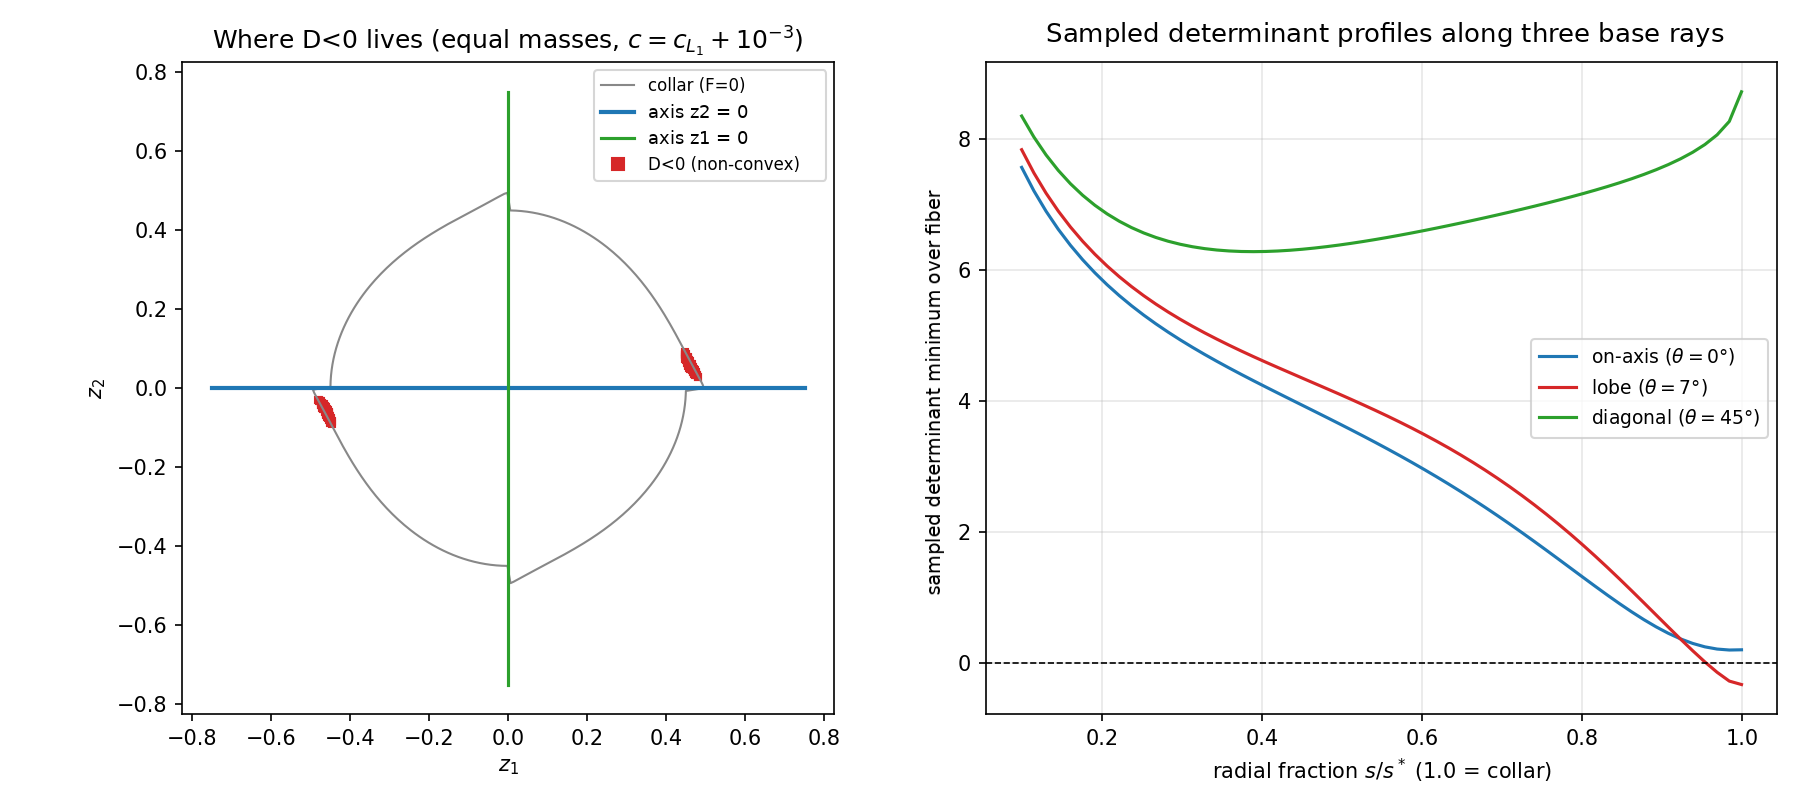
\includegraphics[width=\textwidth]{figures/dynamical_relevance.png}
\caption{Left: sampled negative determinant values near the base collar, with the coordinate axes $z_2=0$ and $z_1=0$. Right: sampled approximations to $D_{\min}$ along three selected rays. These are base-slice profiles, not computed retrograde or direct trajectories. Floating-point, equal masses, $c=c_{L_1}+10^{-3}$.}
\label{fig:relevance}
\end{figure}

We stress the limits of this observation. Dynamical convexity requires an index condition on all contractible closed Reeb orbits, and the rational-section criterion also requires the topology of a proposed binding~\cite{HS}. A positive gate profile on a base axis supplies neither. The sampled lobes identify locations where this embedding-based test detects a problem, but they do not prove dynamical inertness or exclude orbit visits. Nor should the comparable-mass regime be described as wholly unresolved: the near-equal-mass subcritical conclusion is established in~\cite[Thm.~1.16]{LSPCR}.

\subsection{Fine structure of the lobes: a single simple fold}\label{subsec:fold}
A closer look at the lobes records two further numerical regularities, both stable across the comparable-mass band $\mu\in[0.2,0.8]$ (equivalently $m_r\in[0.2,0.8]$) at $c=c_{L_1}+10^{-3}$. They sharpen Observation~\ref{obs:abas} from ``$D_{\min}$ has negative sampled values off-axis'' to a statement about \emph{how} it becomes negative.

\begin{observation}\label{obs:fold}
At the sampled lobe points the reduced tangential gate $\mathcal T$ remains positive: the sampled minimum of $\mathcal T$ over $\{D_{\min}<0\}$ decreases from $+7.5\times10^{-1}$ at $\mu=0.20$ to $+2.6\times10^{-1}$ at $\mu=0.80$, while the sampled minimum of $D_{\min}$ over the same set rises from $-1.69$ to $-1.4\times10^{-3}$ as the lobes shrink. The observed signs are consistent with a \emph{single simple fold}: a negative determinant together with a positive trace corresponds to exactly one negative direction, rather than double concavity. The numerical scans do not certify these signs at every point of the lobes.
\end{observation}

For $F>0$, the matrix $C$ defined in Section~\ref{sec:gates} satisfies $T=4F\tr C$ and $D=4F\det C$. Thus at a fiber direction with $D<0<\calT\le T$, the symmetric matrix $C$ has one positive and one negative eigenvalue. The term \emph{single simple fold} is used here only as a description of this one-negative-direction sign pattern, not as a proved singularity-theoretic normal form. The scans neither certify all points of the lobes nor determine the dynamics there. Figure~\ref{fig:fold} displays the sampled gate profiles.

\begin{figure}[t]
\centering
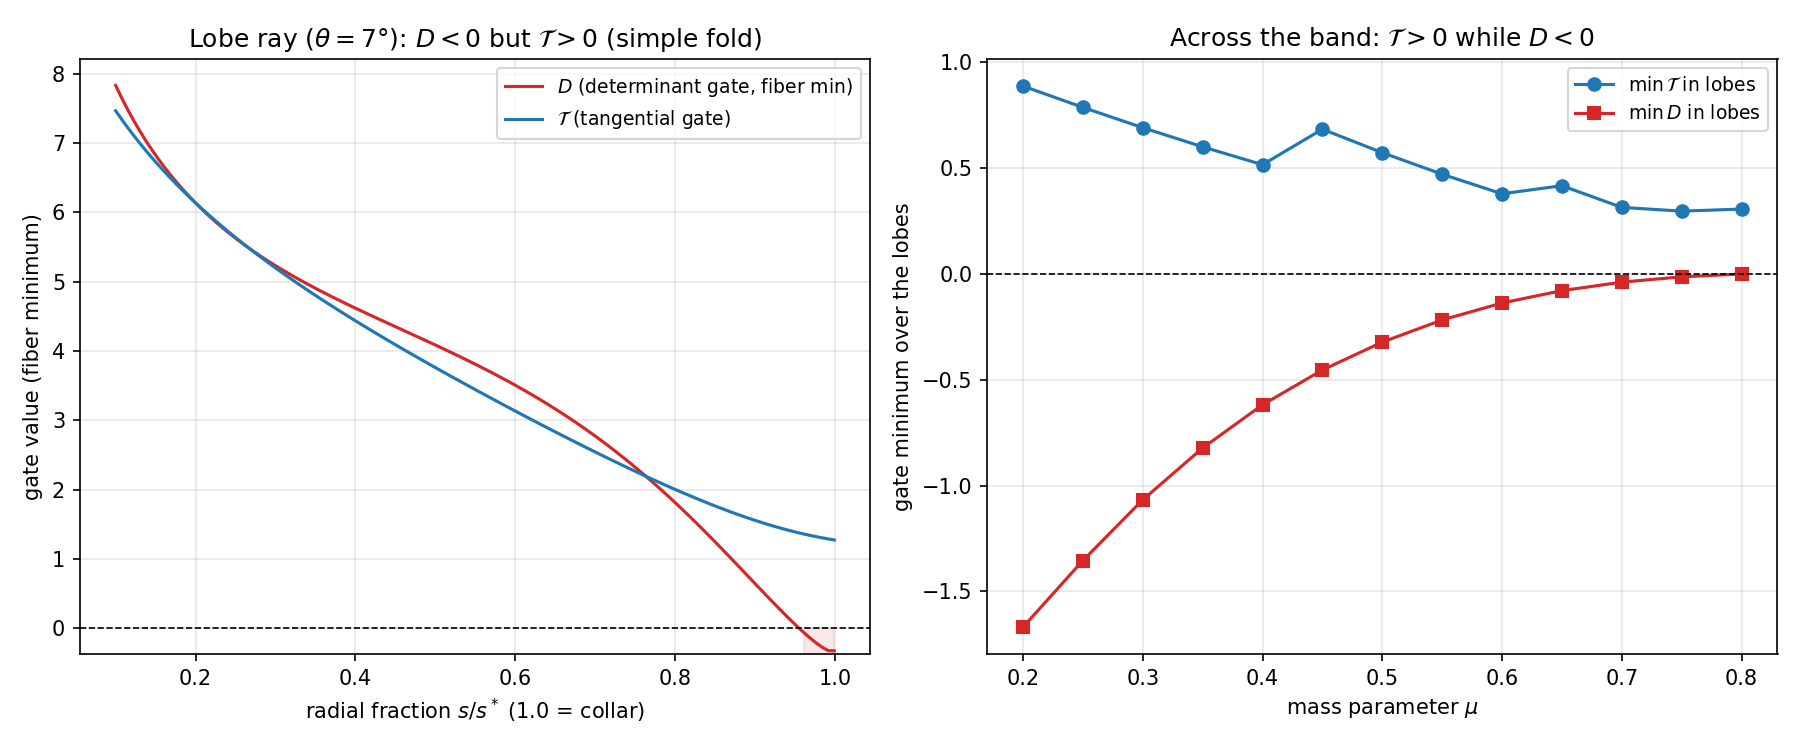
\includegraphics[width=\textwidth]{figures/lobe_structure.png}
\caption{Fine structure of the lobes (floating-point, $c=c_{L_1}+10^{-3}$). Left: along a sampled lobe ray ($\theta=7^\circ$, equal masses), the approximation to $D_{\min}$ dips below zero near the collar while the sampled $\mathcal T$ stays positive. Right: over the sampled mass values and lobe points, the computed minimum of $\mathcal T$ is positive and that of $D_{\min}$ is negative. The labels $D$ in this plot refer to sampled fiber-minimum values, not to the rigorous bound $\calD$.}
\label{fig:fold}
\end{figure}

A companion regularity concerns the radial geometry rather than the fiber. On the sampled rays the computed collar derivative satisfies $\partial F/\partial r<0$ (the collar radial derivative ranges from $-2.5\times10^{-1}$ at $\mu=0.20$ to $-1.0\times10^{-1}$ at $\mu=0.80$), on rays through the lobes no less than on-axis. These values support radial star-shapedness of the bounded base and suggest that the sampled non-convexity lobes do not erode this radial-derivative margin, without identifying radial star-shapedness of this two-dimensional base with contact type of the full regularized hypersurface or with the hypotheses of a global-section theorem~\cite{AFKP,HS}. Both regularities are reproduced by \texttt{code/lobe\_structure.py} in the reproducibility package; like Observation~\ref{obs:abas} they are floating-point at a finite grid and are stated as such.

\section{Limitations and outlook}\label{sec:outlook}

The identities of Section~\ref{sec:elimination} give an exact tangential minimum and a sufficient determinant lower bound. Where both reduced functions are positive, they remove the fiber sweep from the LC-convexity test. The numerical reconnaissance of Section~\ref{sec:map} suggests favorable sampled regimes for light-primary components ($m_r\lesssim 0.045$ near critical, including the Moon component of the Earth--Moon pair), and at energy offsets $\Delta c\gtrsim 0.03$ for the mass values scanned (for the Earth component, $\Delta c\gtrsim 1.2\times 10^{-2}$). Two limitations bound its reach.

First, the reduced determinant gate uses the sufficient condition $\calD>0$, which is sharp only on the collar; away from the collar $\calD$ may be conservative, and a base point with $\calD<0<D_{\min}$ would require the full harmonic minimum of Lemma~\ref{lem:harm} rather than the amplitude bound. This is a matter of tightness, not of correctness.

Second, failure of this LC embedding to be convex must be separated from failure of dynamical convexity or of a global section. The scans suggest a broad near-critical obstruction to this particular convexity test, but they do not certify a continuous parameter boundary. Beyond this test, two approaches are relevant: (i) verifying the required Conley--Zehnder and binding conditions, as in~\cite{HS,LSPCR,LSHill}; and (ii) finding a suitable symplectic embedding, as in the rotating-Kepler and near-equal-mass results~\cite{FKZ,LSPCR}. The near-equal-mass subcritical conclusion of~\cite{LSPCR} is an external result, not a consequence of the present scans. In the midpoint-centered elliptic coordinates $(\lambda,\nu)$ of~\cite{Kim}, the rotation term has the exact identity
\begin{equation}\label{eq:rotation}
(\cosh^2\lambda-\cos^2\nu)\,(q_1 p_2 - q_2 p_1) = \tfrac12\bigl(p_\lambda\sin 2\nu + p_\nu\sinh 2\lambda\bigr),
\end{equation}
a closed form linear in the momenta. In this midpoint-centered convention, adding a nonzero multiple of the rotation term introduces linear momentum terms into the separated Euler Hamiltonian. The mechanical-case curvature argument therefore cannot be applied by substitution without further justification. This identity alone is not a proof of convexity or non-convexity for the rotating model; in particular, a change from midpoint-centered to barycentric coordinates must account for the associated translation terms. The fiber identities of Section~\ref{sec:elimination} remain independent of that outlook. The present reconnaissance supplies no additional orbit-index or global-section theorem.

\section*{Data and Code Availability}

The computational code developed for this study is publicly available on GitHub at \url{https://github.com/cagrisa-creator/pcr3bp-fiber-elimination} (computational baseline version 1.3.2, which implements the mass-convention and scanning corrections described in Section~\ref{sec:map}; the file \texttt{ERRATUM.md} documents the changes, and \texttt{audit/audit\_artigo1.py} independently verifies both the mass convention of Remark~\ref{rem:mass} and the scanning-heuristic failure of version~1). \textbf{Revision-stage note:} A verified Zenodo DOI and an archival release matching the revised manuscript and figure annotations are still pending and must be linked before resubmission.

\appendix

\section{The symbolic audit}\label{app:audit}

The following identities are checked by forming each residual and simplifying it to zero with a computer-algebra system. All eight residuals vanish identically; the driver prints \path{PASS_C82_FIBER_ELIMINATION_AUDIT}. The complete script is included in the reproducibility package as \path{code/fiber_elimination_audit.py}.

\begin{enumerate}
\item[R1] Gap formula~\eqref{eq:Tgap}: $T-\calT-64F^{3/2}(\sqrt s-z_2\cos\phi+z_1\sin\phi)=0$.
\item[R2] Perfect square~\eqref{eq:sq}: $s-(-z_2\cos\phi+z_1\sin\phi)^2-(z_1\cos\phi+z_2\sin\phi)^2=0$.
\item[R3] Attained angle for $s>0$: $\sqrt s-z_2(z_2/\sqrt s)+z_1(-z_1/\sqrt s)=0$. At $s=0$, the angular term vanishes directly, as noted in Lemma~\ref{lem:T}.
\item[R4] Gradient reduction~\eqref{eq:grad}: $|\Fz|^2-(4sF_s^2+8aF_sF_a+4sF_a^2)=0$.
\item[R5] Laplacian reduction~\eqref{eq:lap}: $\Delta F-(4sF_{ss}+8aF_{sa}+4sF_{aa}+4F_s)=0$.
\item[R6] Generic harmonic decomposition~\eqref{eq:harm}: difference of the two sides $=0$ for arbitrary symmetric $L_0,M_1,M_2$, vector $g$, and scalars $\rho,F$.
\item[R7] Determinant sum~\eqref{eq:detsum}: $\det M_1+\det M_2-32s=0$.
\item[R8] Amplitude~\eqref{eq:detsum}: $(\det M_1-\det M_2)^2+\sigma(M_1,M_2)^2-(64s)^2=0$.
\end{enumerate}

Separately, the closed form~\eqref{eq:rotation} for the regularized rotation term in the doubly-covered elliptic coordinates, quoted in Section~\ref{sec:outlook}, is verified both symbolically (residual simplifies to $0$) and numerically (maximum deviation $<10^{-13}$ over $2\times10^5$ random points) by \texttt{code/rotation\_term\_audit.py}, which prints \texttt{PASS\_ROTATION\_TERM\_AUDIT}.

\begin{thebibliography}{10}

\bibitem{AFKP}
P.~Albers, U.~Frauenfelder, O.~van Koert, and G.~P.~Paternain,
\emph{Contact geometry of the restricted three-body problem},
Comm. Pure Appl. Math. \textbf{65} (2012), no.~2, 229--263.

\bibitem{Birkhoff}
G.~D.~Birkhoff,
\emph{The restricted problem of three bodies},
Rend. Circ. Mat. Palermo \textbf{39} (1915), 265--334.
\bibitem{HWZ}
H.~Hofer, K.~Wysocki, and E.~Zehnder,
\emph{The dynamics on three-dimensional strictly convex energy surfaces},
Ann. of Math. (2) \textbf{148} (1998), no.~1, 197--289.

\bibitem{HS}
U.~L.~Hryniewicz and P.~A.~S.~Salom\~ao,
\emph{Elliptic bindings for dynamically convex Reeb flows on the real projective three-space},
Calc. Var. Partial Differential Equations \textbf{55} (2016), no.~2, Art.~43.
\href{https://doi.org/10.1007/s00526-016-0975-x}{doi:10.1007/s00526-016-0975-x}.

\bibitem{Kim}
S.~Kim,
\emph{On a convex embedding of the Euler problem of two fixed centers},
Regul. Chaotic Dyn. \textbf{23} (2018), no.~3, 304--324.\newline
\href{https://doi.org/10.1134/S1560354718030061}{doi:10.1134/S1560354718030061}; arXiv:1701.07258v4.

\bibitem{LeviCivita}
T.~Levi-Civita,
\emph{Sur la r\'egularisation du probl\`eme des trois corps},
Acta Math. \textbf{42} (1920), 99--144.

\bibitem{Salomao2004}
P.~A.~S.~Salom\~ao,
\emph{Convex energy levels of Hamiltonian systems},
Qual. Theory Dyn. Syst. \textbf{4} (2004), 439--454.
\href{https://doi.org/10.1007/BF02970869}{doi:10.1007/BF02970869}.

\bibitem{AFFHvK}
P.~Albers, J.~W.~Fish, U.~Frauenfelder, H.~Hofer, and O.~van Koert,
\emph{Global surfaces of section in the planar restricted 3-body problem},
Arch. Ration. Mech. Anal. \textbf{204} (2012), 273--284.
\href{https://doi.org/10.1007/s00205-011-0475-2}{doi:10.1007/s00205-011-0475-2}.

\bibitem{AFFvK}
P.~Albers, J.~W.~Fish, U.~Frauenfelder, and O.~van Koert,
\emph{The Conley--Zehnder indices of the rotating Kepler problem},
Math. Proc. Cambridge Philos. Soc. \textbf{154} (2013), 243--260.
\href{https://doi.org/10.1017/S0305004112000515}{doi:10.1017/S0305004112000515}.

\bibitem{FKZ}
U.~Frauenfelder, O.~van Koert, and L.~Zhao,
\emph{A convex embedding for the rotating Kepler problem},
arXiv:1605.06981 (2016).

\bibitem{HLS}
U.~L.~Hryniewicz, J.~E.~Licata, and P.~A.~S.~Salom\~ao,
\emph{A dynamical characterization of universally tight lens spaces},
Proc. Lond. Math. Soc. (3) \textbf{110} (2015), no.~1, 213--269.
\href{https://doi.org/10.1112/plms/pdu043}{doi:10.1112/plms/pdu043}.

\bibitem{LSPCR}
L.~Liu and P.~A.~S.~Salom\~ao,
\emph{Finite energy foliations and global dynamics in the restricted three-body problem},
arXiv:2506.17867v2 (2026).

\bibitem{LSHill}
L.~Liu and P.~A.~S.~Salom\~ao,
\emph{Birkhoff conjecture and finite energy foliations in Hill's lunar problem},
arXiv:2606.12912v1 (2026).

\end{thebibliography}

\end{document}
